\chapter{Week 1: Lab Methods and Organelles}\label{Week 1: Lab Methods and Organelles}
% chktex-file 1
% chktex-file 8

\section{Background}\label{Background}
\begin{itemize}
  \item \jjj{Describe the steps in tissue preparation for microscopy:}
    \begin{itemize}
      \item \jjj{Fixation}: typically the first step in the preparation of histological sections in where tissues samples are treated with fixatives as a means to preserve and protect from biological decay.
        \begin{itemize}
          \item \jjj{Fixatives}: solutions, compounds, or others means meant to either disable degradative enzymes, induce cross-linking (stabilizing proteins), or protect from extrinsic damage.
        \end{itemize}
      \item \jjj{Embedding}: the process of placing tissues in a harder medium (e.g., paraffin and plastic resins) as a means to allow for thin slicing of tissue.
        \begin{itemize}
          \item Embedding occurs later in the process of preparation; once a tissue is fixed it must first undergo a series of steps:
          \begin{itemize}
            \item \jjj{Dehydration}: the removal of water using ethanol.
            \item \jjj{Clearing}: replacement of an organic solvent miscible with both alcohol and the embedding medium, giving a translucent appearance.
            \item \jjj{Infiltration}: evaporation of the clearing solvent via exposure to heat (50--\SI{60}{\celsius}) promoting the final embedding of tissue into the medium.
          \end{itemize}
        \end{itemize}
      \item \jjj{Staining}: used as a means to increase contrast in tissue or specific features of tissue that are of interest as most biology tissue has very little inherent contrast.
        \begin{itemize}
          \item \bbb{Basophilic}: dyes that have an affinity for \bbb{anionic} (net \bbb{negative} charge) cells parts.
            \begin{itemize}
              \item E.g., hematoxylin, toluidine blue, alcian blue, and methylene blue.
            \end{itemize}
          \item \rrr{Acidophilic}: dyes that have an affinity for \rrr{cationic} (net \rrr{positive} charge) cell parts.
            \begin{itemize}
              \item E.g., eosin, orange G, and acid fuchsin
            \end{itemize}
        \end{itemize}
    \end{itemize}
  \item \jjj{What does H \& E Stain?}
    \begin{itemize}
      \item \chap{Hematoxylin (H)} and \amp{eonsin (E)} stains are among the most commonly used stains. 
        \begin{itemize}
          \item As mentioned above, hematoxylin acts as a \bbb{basophilic dye}, turning negatively charge organelles like the cell nucleus, RNA-rich regions of cytoplasm, cartilage, anywhere from \bbb{blue} \chap{\to} \xxx{purple}.
          \item Eosin acts as an \rrr{Acidophilic dye}, typically turning \amp{cationic structures pink}; sometimes it is considered to be a \jjj{counterstain}, i.e., typically a secondary dye that is meant to distinguish features.
        \end{itemize}
    \end{itemize}
  \item \jjj{What does PAS Stain?}
    \begin{itemize}
      \item \xxx{Periodic acid-Schiff (PAS)} utilizes hexose rings of polysaccharides and other carbohydrate rich structures to stain macromolecules \xxx{purple} \to~\fff{magenta}.
    \end{itemize}
  \item \jjj{Describe Enzyme Histochemistry.}
    \begin{itemize}
      \item Enzyme histochemistry is a method for localizing cellular structures using specific enzymatic activity in such structures.
      \item Preservation of enzymes often requires non-fixed or mildly fixed tissue and generally adhere to the following steps:
        \begin{enumerate}
          \item Tissues sections are immersed in solution containing the substrate of the enzyme to be localized.
          \item The enzyme is exposed to and allowed to act on the substrate.
          \item A marker compound is introduced and reacted with the product from step 2.
          \item Location is determined via precipitation of the insoluble product, which must be visible a light or electron microscopy, over the site of the enzyme.
        \end{enumerate}
      \item Phosphatase, dehydrogenase, and peroxidase are common examples of enzymes detected with histochemistry.
    \end{itemize}
  \item \jjj{How does Immunohistochemistry work?}
    \begin{itemize}
      \item Immunohistochemistry (IHC): the use of labeled antibodies and antigens to identify and localize many proteins and macromolecules that lack specific enzymatic activity. 
      \item Visualization of such interactions are commonly  accomplished with either:
        \begin{itemize}
          \item Chromogenic immunohistochemistry (CIH): use of antibodies conjugated to an enzyme that catalyzes a color-producing reaction.
          \item Immunofluorescence: tagging of a fluorophore (fluorescein, rhodamine) to an antibody. 
        \end{itemize}
      \item Common used in diagnosis of abnormal cells such as those in cancerous tumors. 
    \end{itemize}
\end{itemize}

\section{Microscopic Techniques}
\begin{itemize}
  \item \jjj{Bright field}: a very common method that uses ordinary light and stained structures to discern differences and cell structures. 
  \begin{center}
    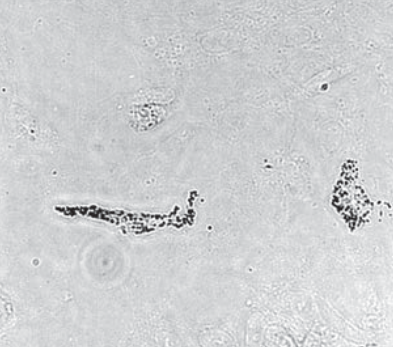
\includegraphics[scale=0.45]{images/week-1-1a.png}
  \end{center}
  \item \jjj{Phase contrast}: uses differences in refractive index of natural cell and tissue components; allows for observation of living cells.
  \begin{center}
    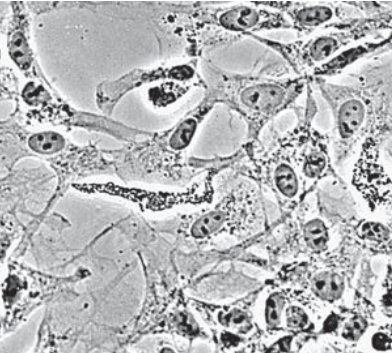
\includegraphics[scale=0.45]{images/week-1-1b.png}
  \end{center}
  \item \jjj{Confocal}: use of scans at successive focal planes with a more focused light beam, usually from a laser, to construct a 3D image.
  \begin{center}
    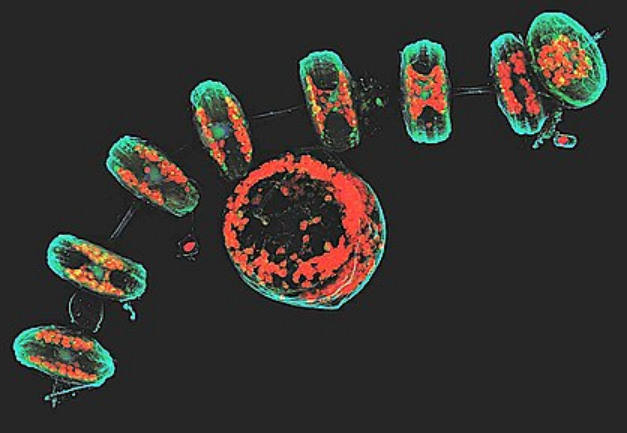
\includegraphics[scale=0.50]{images/week-1-1c.png}
  \end{center}
  \item \jjj{Fluorescent}: use of longer wavelengths emitted via specific perturbations of cellar substances using a specific wavelength (usually UV). Useful for identification of cells and components that have affinity for specific fluorescent compounds. 
  \begin{center}
    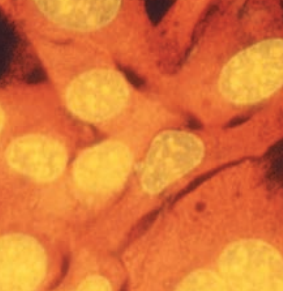
\includegraphics[scale=0.60]{images/week-1-1d.png}
    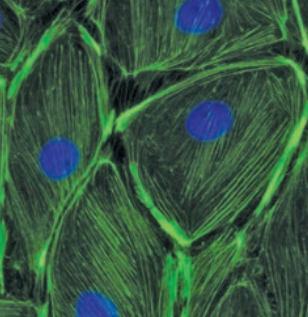
\includegraphics[scale=0.55]{images/week-1-1e.png}
  \end{center}
  \newpage
  \item \jjj{Transmission Electron Microscopy (TEM)}: a high resolution (3 nm) that allows for particles to be magnified many times via transmission of electrons though a specimen; very thin tissue sections are used and a flat image is made from the intersection of the electron beam and the sample.
  \begin{center}
    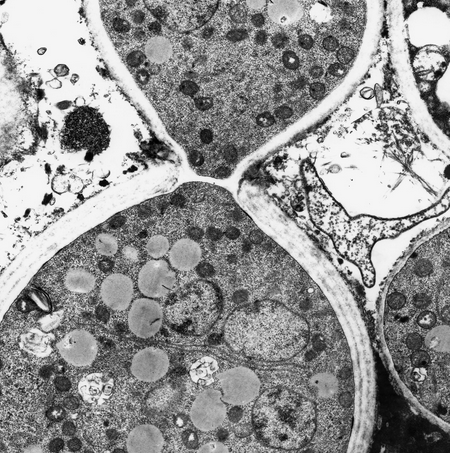
\includegraphics[scale=0.60]{images/week-1-1g.png}
  \end{center}
  \item \jjj{Scanning Electron Microscopy (SEM)}: used to provide a high resolution view of the surface of cells, tissues, and organs. Unlike TEM, SEM does not intersect with the specimen, instead the electrons are reflected by a coating and then collected, analyzed, and used to generate a 3D view.
  \begin{center}
    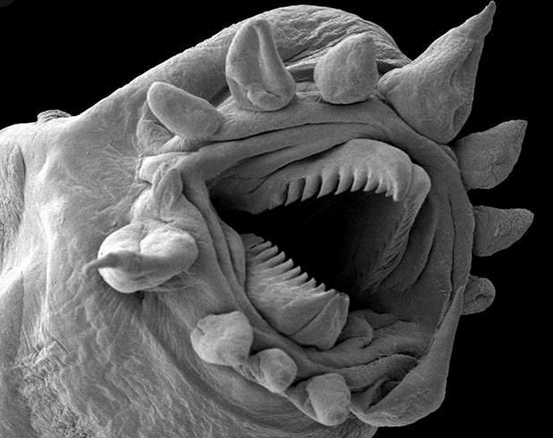
\includegraphics[scale=0.60]{images/week-1-1f.png}
  \end{center}
\end{itemize}
\clearpage
\section{Organelles and Cytoplasmic Inclusions}
\begin{multicols}{2}
\begin{itemize}
  \item \jjj{Nucleus}: a large membrane bound organelle that contains chromatin, the nucleolus, and nucleoplasm. \\ 
  \textit{Size}: \emph{5--20 \si{\micro m}}, the largest organelle. \\
  \begin{center}
    \hspace{-30pt}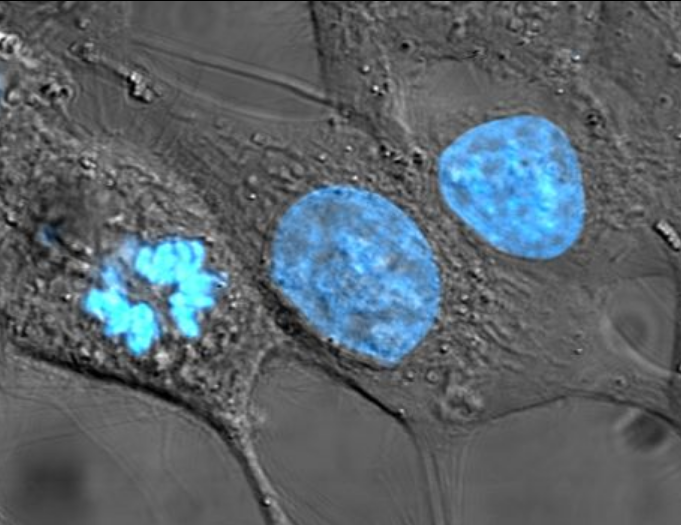
\includegraphics[width=0.65\columnwidth]{images/week-1-nucleus.png}
  \end{center}
  \item \jjj{Nucleolus}: large, dense structure within the nucleus that functions in the synthesis of ribosomes. \\
  \textit{Size}: \emph{0.5--5 \si{\micro m}}, smaller than nucleus.
  \begin{center}
    \hspace{-30pt}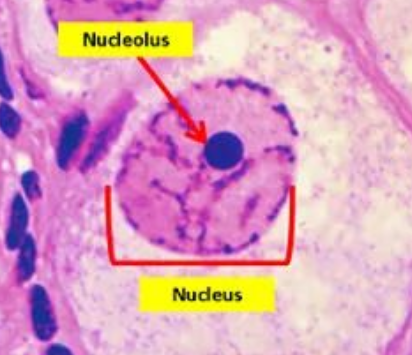
\includegraphics[width=0.65\columnwidth]{images/week-1-nucleolus.png}
  \end{center}
  \item \jjj{Plasma Membrane}: phospholipid bilayer containing various elements, acts as a physical barrier to regulate internal environment; maintains charge and functions in cell communication. \\
  \textit{Size}: \emph{5--10 \si{nm}}, very thin---3 orders of magnitude less than width of nucleus.
  \begin{center}
    \hspace{-30pt}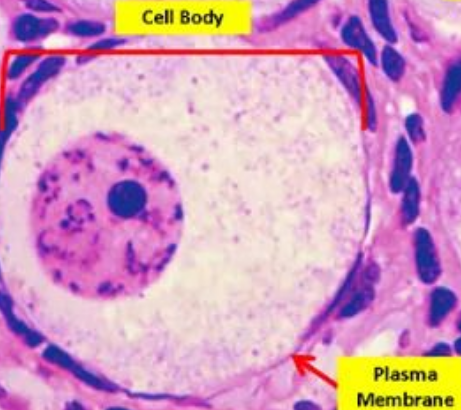
\includegraphics[width=0.65\columnwidth]{images/week-1-plasma.png}
  \end{center}
  \item \jjj{Rough ER}: interconnect membrane that modifies, transports, and stores proteins produced by attached ribosomes. \\
  \textit{Size}: \emph{5--8 \si{nm} thick, \emph{20-30 \si{nm} wide}}, membrane of rER thin, while the lumen is wide and surrounds nucleus (often).
  \begin{center}
    \hspace{-30pt}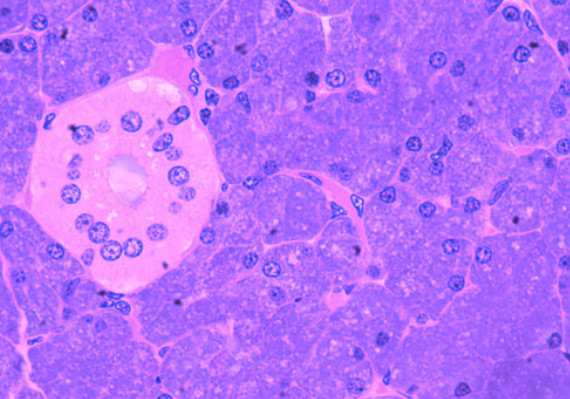
\includegraphics[width=0.65\columnwidth]{images/week-1-rer.png}
  \end{center}
  \item \jjj{Smooth ER}: Like rER, but lacking ribosomes; synthesizes, transports, and stores lipids; metabolizes carbohydrates, toxins (of various types); and forms vesicles and peroxisomes.\\
  \textit{Size}: lumen is \emph{30--60 \si{nm}} thick, larger than rER\@; overall fraction of cell varies.
  \begin{center}
    \hspace{-30pt}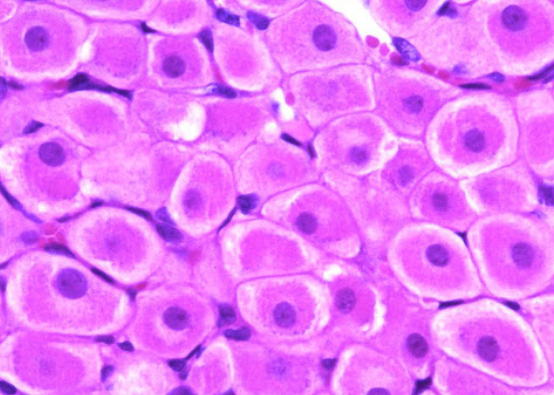
\includegraphics[width=0.65\columnwidth]{images/week-1-ser.png}
  \end{center}
  \item \jjj{Golgi Apparatus}: modifies, packages, and sorts materials that arrive from the ER; forms secretory vesicles/lysosomes. \\
  \textit{Size}: \emph{2--5 \si{mm}}, stacks of flat membranes, can occupy large portion of cell.
  \begin{center}
    \hspace{-30pt}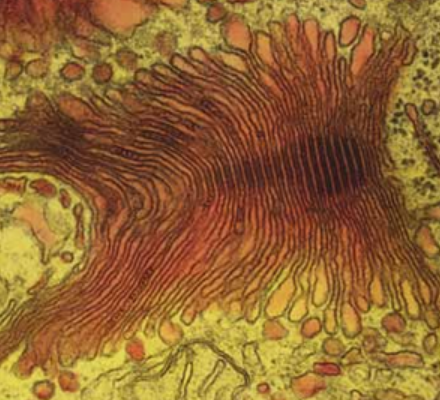
\includegraphics[width=0.6\columnwidth]{images/week-1-golgi.png}
  \end{center}
  \item \jjj{Vesicles}: \\
  \textit{Size}: \emph{30--100 \si{nm}}, large range varies among different types of vesicles, still relatively small.
  \begin{center}
    \hspace{-30pt}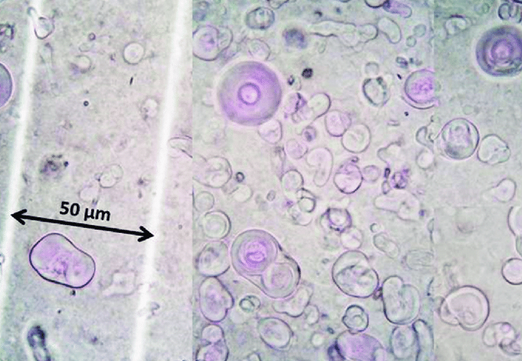
\includegraphics[width=0.75\columnwidth]{images/week-1-vesicle.png}
  \end{center}
  \item \jjj{Mitochondria}: \\
  \textit{Size}: \emph{0.5--1 \si{\micro m}}, decently sized, but still smaller than other organelles in the cell.
  \begin{center}
    \hspace{-30pt}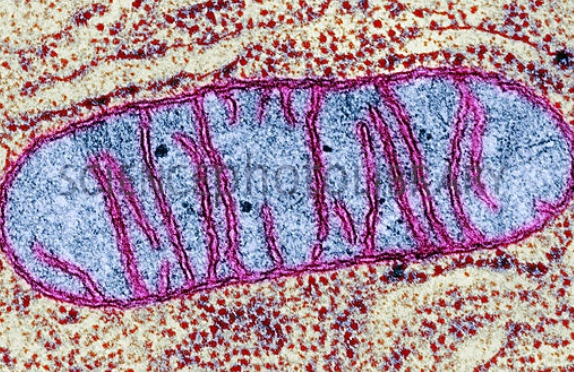
\includegraphics[width=0.75\columnwidth]{images/week-1-powerhouse.png}
  \end{center}
  \item \jjj{Endosomes}: collection of intracellular sorting organelles, originating from trans Golgi network that move molecules and ligands to lysosomes (L), or recycled back to cell membrane.\\
  \textit{Size}: \emph{1--50 \si{\micro m}}, depends on stage;\\
  (E)rly forms dynamic tubular network, can be long. % chktex 36
  (M)vbs (late) lack tubes.\\ % chktex 36
  TEM, not light microscope below*
  \begin{center}
    \hspace{-30pt}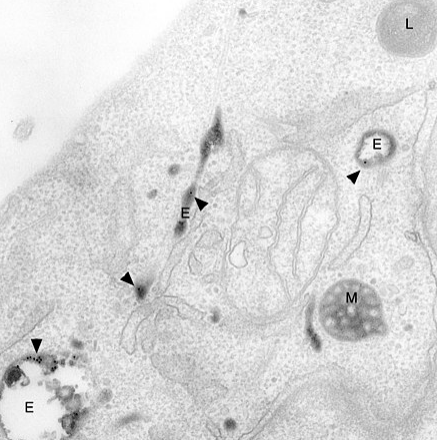
\includegraphics[width=0.75\columnwidth]{images/week-1-endosome.png}
  \end{center}
  \item \jjj{Lysosomes}: spherical-shaped from Golgi, contains digestive enzymes to break down microbes and materials.\\
  \textit{Size}: \emph{0.5--1 \si{\micro m}}, rather small, TEM used below instead of light microscope.
  \begin{center}
    \hspace{-30pt}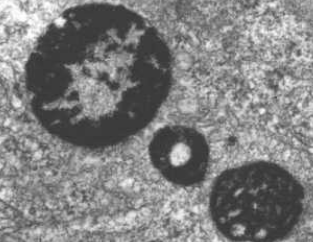
\includegraphics[width=0.69\columnwidth]{images/week-1-lysosome.png}
  \end{center}
  \item \jjj{Peroxisomes}: formed via ER or fission; contains enzymes to break down specific harmful substances, also used for beta oxidation of fatty acids. \\
  \textit{Size}: \emph{0.1--1 \si{\micro m}}, typically smaller than lysosomes, can be similar sized.
  \begin{center}
    \hspace{-30pt}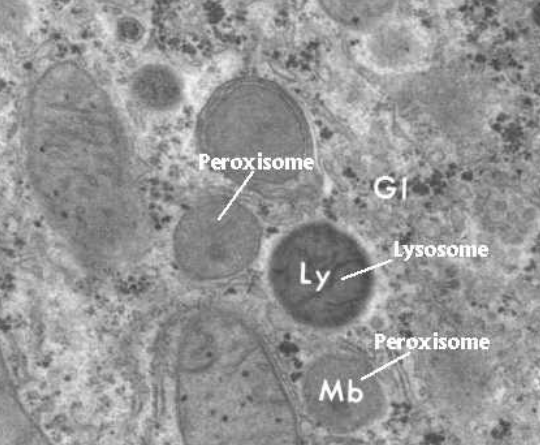
\includegraphics[width=0.69\columnwidth]{images/week-1-peroxisome.png}
  \end{center}
  \item \jjj{Cytoskeleton}: organized network of \{actin, micro-, intermediate\} filaments, and microtubules and other proteins.\\
  \textit{Size}: \emph{7 \si{nm}}, varies, depending on structure and filaments used.
  \begin{center}
    \hspace{-30pt}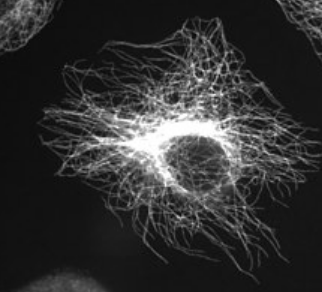
\includegraphics[width=0.69\columnwidth]{images/week-1-cytoskeleton.png}
  \end{center}
  \item \jjj{Ribosomes}: composed of protein and rRNA and engage in protein synthesis; can be on rER, in plasma membrane, in lysosomes, and free in cell. \\
  \textit{Size}: \emph{20--30 \si{nm}}, varies, organized into both large and small subunits.
  \begin{center}
    \hspace{-30pt}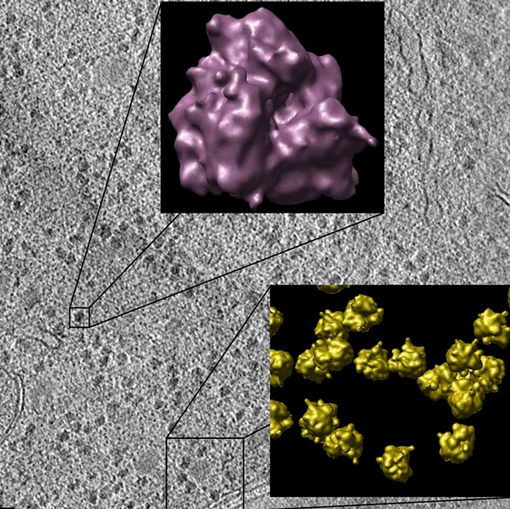
\includegraphics[width=0.8\columnwidth]{images/week-1-ribosome.png}
  \end{center}
  \item \jjj{Glycogen granules}: aggregates of carbohydrate polymer in which glucose is stored, notably in liver cells\\
  \textit{Size}: \emph{20--30 \si{\micro m}}, many can cluster.
  \begin{center}
    \hspace{-30pt}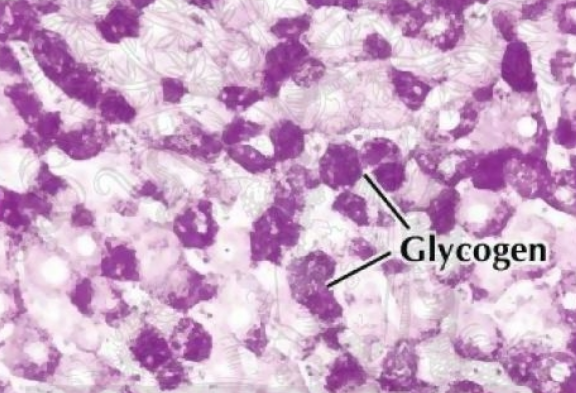
\includegraphics[width=0.8\columnwidth]{images/week-1-glycogen.png}
  \end{center}
  \item \jjj{Liquid droplets}: accumulations of lipid-filling adipocytes. \\
  \textit{Size}: \emph{20--30 \si{\micro m}}, can be removed.
  \begin{center}
    \hspace{-30pt}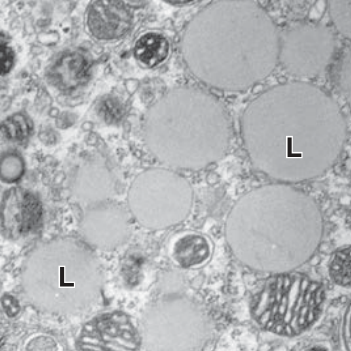
\includegraphics[width=0.8\columnwidth]{images/week-1-liquid.png}
  \end{center}
  \end{itemize}
\end{multicols}
  \subsection{Labeled Diagram of a Eukaryotic Cell}
  \begin{figure*}[h]
    \centering
    \def\svgwidth{\textwidth}
    \input{images/animal-cell.pdf_tex}
  \end{figure*}


  \clearpage
  \section{Mitotic Phases}
  \begin{center}
    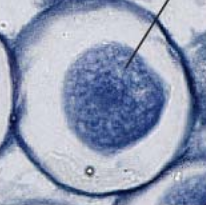
\includegraphics[scale=0.5]{images/week-1-mp1.png}
  \end{center}
  \begin{itemize}
    \item 
  \end{itemize}
  \begin{center}
    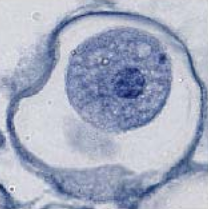
\includegraphics[scale=0.5]{images/week-1-mp2.png}
  \end{center}
  \begin{itemize}
    \item 
  \end{itemize}
  \begin{center}
    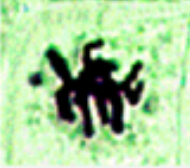
\includegraphics[scale=0.5]{images/week-1-mp3.png}
  \end{center}
  \begin{itemize}
    \item 
  \end{itemize}
  \begin{center}
    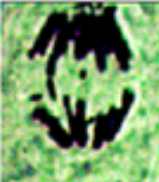
\includegraphics[scale=0.5]{images/week-1-mp4.png}
  \end{center}
  \begin{itemize}
    \item 
  \end{itemize}
  \begin{center}
    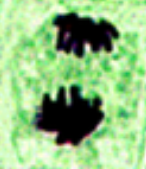
\includegraphics[scale=0.5]{images/week-1-mp5.png}
  \end{center}
  \begin{itemize}
    \item 
  \end{itemize}

  
\section{Apoptosis Events}\label{Apoptosis Events}
\begin{itemize}
  \item \jjj{DNA fragmentation}:
  \item \jjj{Decrease of cell volume}:
  \item \jjj{Membrane Blebbing}:
  \item \jjj{Formation of apoptotic bodies}:
\end{itemize}

\section{Features and Functions}
\begin{itemize}
  \item \jjj{Stratified squamous epithelium}:
  \begin{itemize}
    \item Features:
    \item Functions:
  \end{itemize}
  \item \jjj{Simple cuboidal epithelium}:
  \begin{itemize}
    \item Features:
    \item Functions:
  \end{itemize}
  \item \jjj{Skeletal muscle}:
  \begin{itemize}
    \item Features:
    \item Functions:
  \end{itemize}
  \item \jjj{Cardiac muscle}:
  \begin{itemize}
    \item Features:
    \item Functions:
  \end{itemize}
  \item \jjj{Smooth muscle}:
  \begin{itemize}
    \item Features:
    \item Functions:
  \end{itemize}
\end{itemize}